\documentclass{standalone}
\usepackage{pgfplots}
\pgfplotsset{compat=newest}

\begin{document}
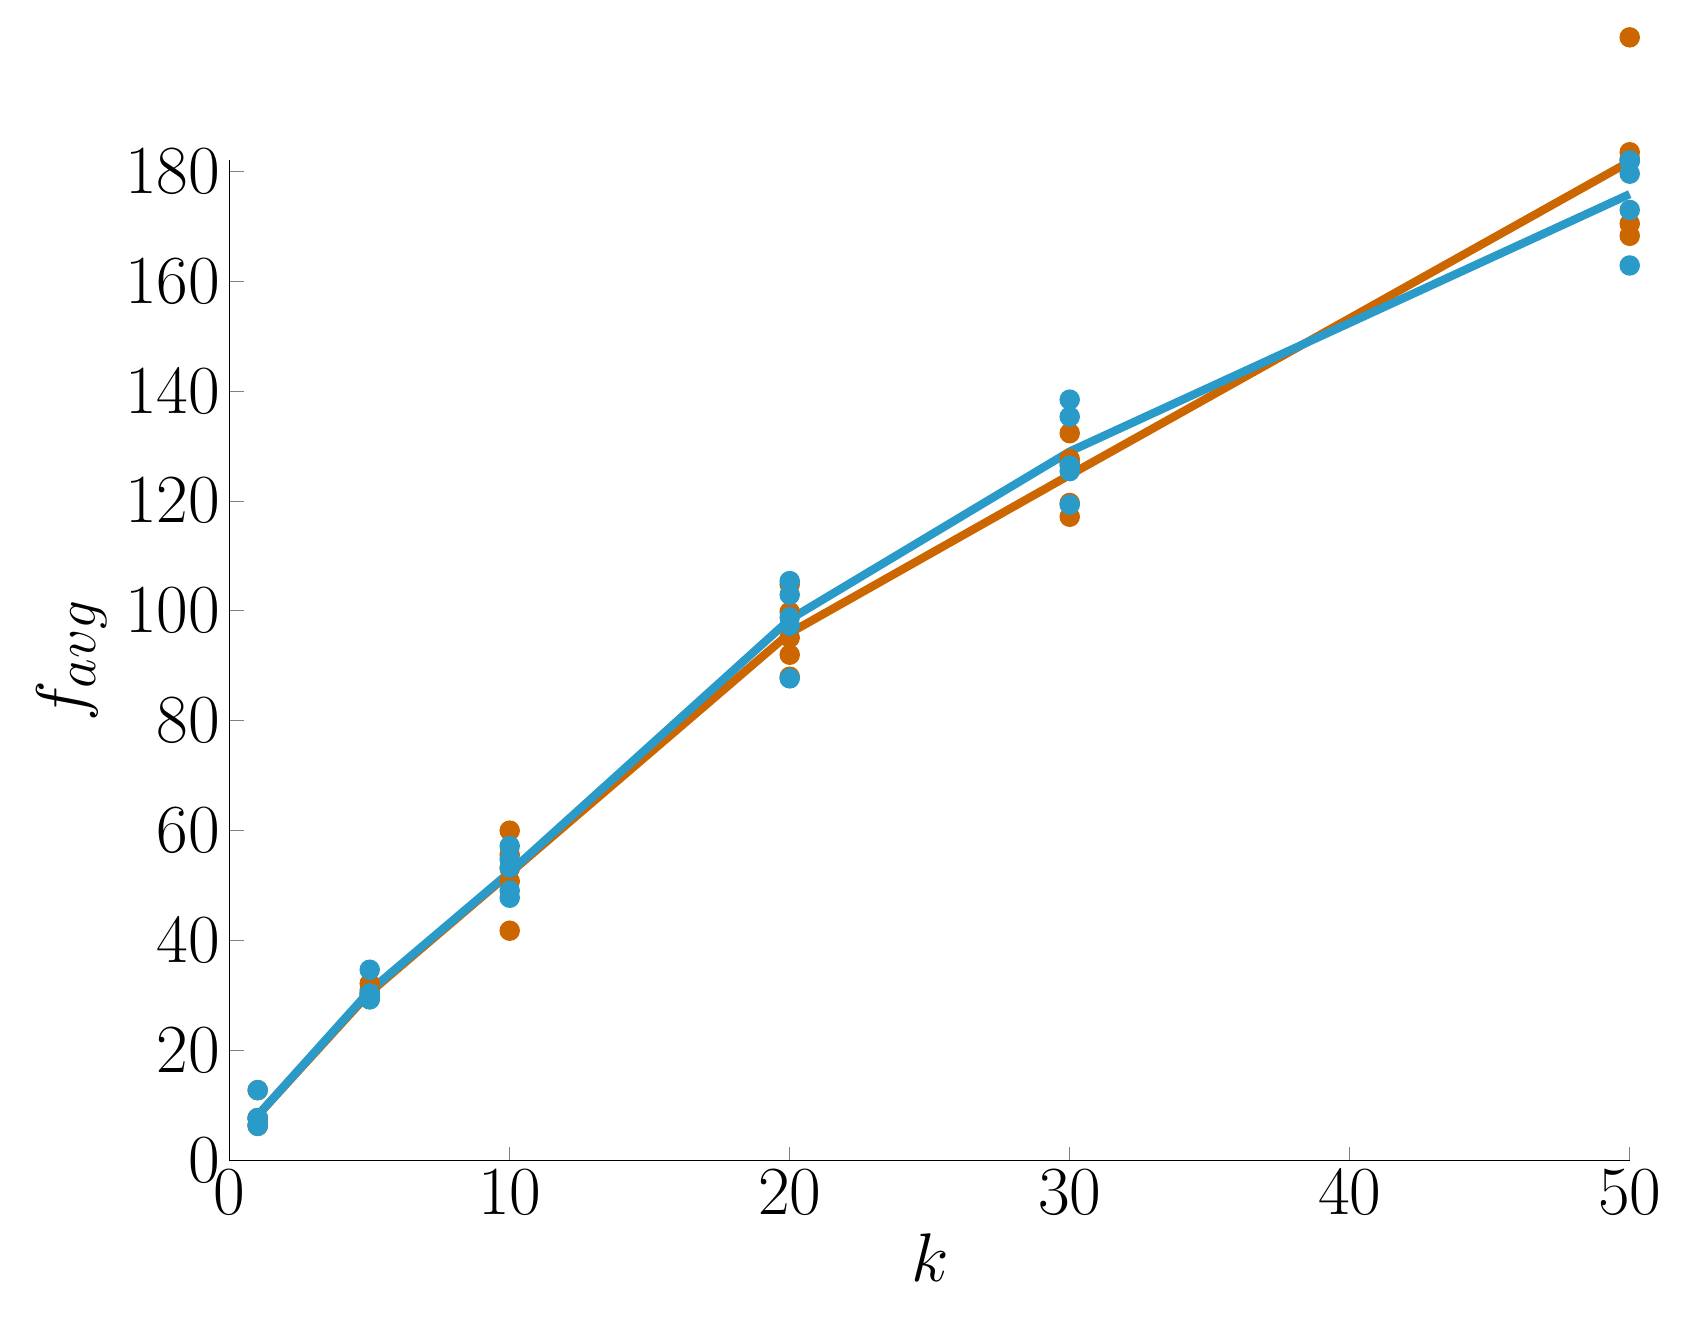
\begin{tikzpicture}

\begin{axis}[%
tick label style={font=\Huge},
label style={font=\Huge},
legend style={font=\Huge},
view={0}{90},
max space between ticks=50pt,
width=7in,
height=5in,
scale only axis,
xmin=0, xmax=50,
xtick={0, 10, 20, 30, 40, 50},
xlabel={$k$},
ymin=0, ymax=181.9,
%ytick={0, 200, 400, 600, 800, 1000},
ylabel={$f_{avg}$},
major tick length=5pt,
axis lines*=left,
legend cell align=left,
clip=false]

\addplot [
only marks,
mark=*,
mark size=3.5pt,
color=orange!80!black,
%solid,
%line width=2pt,
]
coordinates{
(1,6.3)(1,6.5)(1,7.7)(1,7.7)(1,12.8)(5,29.4)(5,29.7)(5,30.4)(5,31.0)(5,32.2)(10,41.8)(10,50.8)(10,53.1)(10,55.6)(10,60.0)(20,88.0)(20,92.0)(20,95.1)(20,99.8)(20,104.8)(30,117.1)(30,119.6)(30,126.9)(30,127.6)(30,132.3)(50,168.2)(50,170.4)(50,182.2)(50,183.4)(50,204.3)
};

\addplot [
only marks,
mark=*,
mark size=3.5pt,
color=cyan!80!black,
%solid,
%line width=2pt,
]
coordinates{
(1,6.3)(1,6.5)(1,7.7)(1,7.7)(1,12.8)(5,29.3)(5,29.8)(5,30.1)(5,30.4)(5,34.7)(10,47.8)(10,49.1)(10,53.3)(10,54.8)(10,57.2)(20,87.7)(20,97.3)(20,98.8)(20,102.9)(20,105.4)(30,119.3)(30,125.4)(30,126.4)(30,135.3)(30,138.4)(50,162.8)(50,172.9)(50,179.5)(50,181.8)(50,181.9)
};

\addplot [
color=orange!80!black,
solid,
line width=3pt
]
coordinates{
(1,8.2)(5,30.54)(10,52.26)(20,95.94)(30,124.7)(50,181.7)
};

\addplot [
color=cyan!80!black,
solid,
line width=3pt
]
coordinates{
(1,8.2)(5,30.86)(10,52.44)(20,98.42)(30,128.96)(50,175.78)
};


\end{axis}
\end{tikzpicture}
\end{document}
